\documentclass[12pt]{ociamthesis}  % default square logo 
%\documentclass[12pt,beltcrest]{ociamthesis} % use old belt crest logo
%\documentclass[12pt,shieldcrest]{ociamthesis} % use older shield crest logo

%load any additional packages
\usepackage{amssymb}
\usepackage{amsmath}
\usepackage{float}

%input macros (i.e. write your own macros file called mymacros.tex 
%and uncomment the next line)
%\include{mymacros}

\title{Optimizing Vortex Methods for Real-Time Wake Simulation}   %note \\[1ex] is a line break in the titlehttps://preview.overleaf.com/public/wvmhnwxnkknq/images/6f5f6fdd1d6f308adb5eddffc3c297d242a47056.jpeg

\author{Sebastian Preston-Jensen}             %your name
\college{School of Mechanical, Aerospace and Civil Engineering}  %your college

%\renewcommand{\submittedtext}{change the default text here if needed}
\degree{Individual Project}     %the degree
\degreedate{2016-2017}         %the degree date

%end the preamble and start the document
\begin{document}

%this baselineskip gives sufficient line spacing for an examiner to easily
%markup the thesis with comments
\baselineskip=18pt plus1pt
\numberwithin{equation}{section}

%set the number of sectioning levels that get number and appear in the contents
\setcounter{secnumdepth}{4}
\setcounter{tocdepth}{3}


\maketitle                  % create a title page from the preamble info
\include{dedication}        % include a dedication.tex file
\include{acknowlegements}   % include an acknowledgements.tex file
\include{abstract}          % include the abstract

\begin{romanpages}          % start roman page numbering
\tableofcontents            % generate and include a table of contents
\listoffigures              % generate and include a list of figures
\end{romanpages}            % end roman page numbering

%now include the files of latex for each of the chapters etc
\section{Introduction}
\subsection{Overview}
The aim of this project was to develop a Discrete Vortex Method (DVM) simulation capable of running in real-time to simulate the vortex wakes produced by an aircraft during flight. The DVM was programmed in Unity using C-Sharp. The simulation was split into 3 main functions; the Convective Scheme, the Discretization Scheme and Supporting Infrastructure. Each segment was investigated and optimized separately.
\\\\
The movement of air in the wake region left behind an aircraft poses a potential risk to other aircraft. As such, wake regions are implicated as the main contributing factor in many aircraft crashes. The most notable of these crashes is Delta Air Lines Flight 9570, where a McDonald Douglas DC-9, a mid size passenger plane, rotated suddenly around its roll axis during landing, causing a collision with the runway. The crash was fatal for all occupants of the plane. The NTSB (National Transport Safety Bureau) investigation into the crash accounts the sudden rolling of the aircraft to the planes interaction with the wake region caused by a larger DC-10 aircraft that had landed moments before.
\\\\
To avoid such crashes the NTSB mandated stricter wake-separation periods. Wake-Separation periods are waiting times between which subsequent aircraft landing on the same runway must wait. These waiting times represent a significant contribution to limiting airport capacity. Thus vortex wake regions are implicated in safety and efficiency concerns.

\subsection{Motivations/Uses}
The overview section provided an introduction to vortex wake and their implications to society. This section serves to outline the potential uses of a simulation of vortex wakes capable of running in real-time.
\\\\
As previously discussed, vortex wakes pose a significant safety concern if a plane enters the wake region. One way to improve the safety in such situations would be to increase the pilots competence at handling such a situation. This is of up most important if the pilot is required to fly in conditions where vortex wake interactions are unavoidable, EG air-to-air refueling. Training pilots in a real-life situation is both impractical and dangerous. Use of a flight simulator remedies both these concerns, however flight simulators employed in current pilot training implement limited and simplistic aerodynamic models. The realism, and therefore usefulness, of such simulators could be improved via implementation of a simulation of the vortex wakes regions such as the one developed for this project. Flight simulators must operate in real-time to provide an imersive experience for the pilot, hence is it imperative that the simulation be capable of running in real-time.
\\\\
Vortex wakes are not immediately apparent as they cannot be seen. Safety could therefore be improved if a pilot could visualize vortex wakes. Such a system be devised using the output of a simulation capable of running in real-time. 
\\\\
Wake-Separation periods are a major contribution to limiting airport capacity. Separation periods are mandated in order to ensure the safety of landing aircraft. Separation periods currently consist of imposing a set waiting period, dependent on the size of aircraft previously landed, until the runway may be used again. These separation periods are specified to be applicable to all situations an aircraft controller may experience, hence they often overestimate the time required for the runaway to become safe again. If separation periods can be reduced safely airport capacity can increased, further aircraft may be able to spend less time circling the airport and thus burn less fuel, lessening their impact on the environment. If an air traffic controller was equipped with a simulation that predicted the wake of aircraft landing with a high enough degree of accuracy, wake separation times could be decreased.
\\\\
If the simulation can be run quicker than real-time then the simulation could be used as a predictive tool. For example, air traffic controllers could predict the wake regions behind planes near their airports at points in the future and identify problematic interactions before they arise and adjust the bearings of planes accordingly.

\subsection{Literature Review}

\subsection{Report Format}
This report is organized in 5 main sections; Introduction, Theory, Methods, Results and discussion.
%\section{Simulation Architecture}
\subsection{Introduction}

\section{Theory - Convection Schemes}
\subsection{Introduction}
The convective scheme is responsible for calculating the velocities of all Discrete Vortex Elements given the velocity fields induced by all other elements. The velocity field due to a vortex at any given point is given by the Biot-Savart law, shown in equation \ref{eq:convbase1}

\begin{equation}
\label{eq:convbase1}
\vec{V}(x,y,z)=\frac{\Gamma}{4\pi}\int_{+\infty}^{-\infty} \frac{d\vec{\ell}\times\vec{r}}{|\vec{r}|^3}
\end{equation}

To calculate the velocity field at any given point, the influence of all vortex elements must be taken into account, this is found via the summation of the influences of all elements (representing filaments) found through the Biot-Savart law. This is represented in equation \ref{eq:convbase2} where $N$ is the total amount of elements, and $n$ is the individual element being considered

\begin{equation}
\label{eq:convbase2}
\vec{V}(x,y,z)=\sum_{n=1}^{N} \frac{\Gamma}{4\pi}\int_{+\infty}^{-\infty} \frac{d\vec{\ell_n}\times\vec{r_n}}{|\vec{r_n}|^3}
\end{equation}

The computational cost of a single evaluation of the Biot-Savart law does not change meaningfully for different variables input into equation \ref{eq:convbase1}, the maths required is constant but slight variations may arise from larger inputs. Hence, making the assumption that the computational cost of a single evaluation of the Biot-Savart law is constant, we can express the computational cost as in equation \ref{eq:convbase3} where $C_{Inv}(x,y,z)$ is the computational cost due to a single element at a given point and $A$ is a constant.

\begin{equation}
\label{eq:convbase3}
C_{Single}(x,y,z)=A
\end{equation}

From the expression in equation \ref{eq:convbase3} we can form an expression for the velocity field induced by all elements, this is shown in equation \ref{eq:convbase4}

\begin{equation}
\label{eq:convbase4}
C_{Total}(x,y,z)=\sum_{n=1}^{N} C_{Inv}(x,y,z)=NA
\end{equation}

From equation \ref{eq:convbase4} it can be seen that the complexity of calculating the velocity field is linearly proportional to the amount of elements present. The velocity of an element is found by evaluating the velocity field at that elements position. A single iteration of the convection scheme must calculate the velocity of all elements present, an expression for the computational cost is given in equation \ref{eq:convbase5}

\begin{equation}
\label{eq:convbase5}
C_{Iteration}=\sum_{n=1}^{N} C_{Total}(x_n,y_n,z_n)\approx AN^2
\end{equation}

Equation \ref{eq:convbase5} shows that the computational cost of calculating the new velocities of all elements present increases in complexity proportional to $N^2$. This is known mathematically as an N-Body problem. The computational cost of a single evaluation of the Biot-Savart law, A, is fixed. However modifying the way in which the law is applied constitutes the basis for more computationally efficient convective schemes.
\\\\
In this section, two modifications to the convective scheme are suggested and evaluated. Both schemes necessarily introduce errors into the numerical solution. The schemes are evaluated based upon a consideration of their performance and accuracy

\subsection{Biasing}
Biasing is the simplest method of optimization for the convection scheme. Biasing works by "biasing" which elements are taken into account when convecting a given element. Consider again the Biot-Savart law, shown in equation \ref{eq:bias1} for clarity.

\begin{equation}
\label{eq:bias1}
\vec{V}(x,y,z)=\frac{\Gamma}{4\pi}\int_{+\infty}^{-\infty} \frac{d\vec{\ell}\times\vec{r}}{|\vec{r}|^3}
\end{equation}

From equation \ref{eq:bias1} two things can be noted, the influence of an element on a given element is majorly dependent only on two variables, the convecting elements vorticity $\Gamma$ and the its distance vector $\vec{r}$. Biasing methods exploit these relationships by ignoring the convective effects of an element if its influence on a certain element can be considered negligible. 
\\\\
Determining whether or not an elements influence is negligible requires an evaluation of either the vorticity $\Gamma$ or distance vector $\vec{r}$ of the given element, or a coefficient based upon both of these. This evaluation must be performed for all elements every time an element is convected, so the evaluation must be performed $N^2$ times per iteration, an equal amount of times as the Biot-Savart law must be evaluated in the absence of a biasing scheme. It is also important to note that this evaluation process must be performed even for elements whose effects will be taken into account. The evaluation scheme must therefore be kept lightweight and efficient in order to pose a performance increase of the scheme. If a computationally costly evaluation process is used it may pose a decrease in both overall performance and accuracy of the simulation.
\\\\
The simplest biasing system would make an evaluation based upon both Vorticity and distance vector, such an evaluation is shown in the condition in equation \ref{eq:bias2} where A is an arbitrary constant.

\begin{equation}
\label{eq:bias2}
\frac{\Gamma}{\vec{r}}>A
\end{equation}

This approach provides the most accurate results, however it is also the most computationally expensive as it involves both an evaluation and a calculation. Two other criteria may be used for biasing the effect of elements based solely on distance and vorticity respectively. Evaluations based on on either vorticity or distance have the advantage of being more lightweight and representing an almost negligible overhead Whether it is best to consider vorticity or distance depends on the situation that need be modeled. A situation where all elements are close would likely benefit more from an evaluation based on vorticity, however an application where elements are spaced with a larger distance may benefit from an evaluation based on distance.
\\\\
The simulation considered here is of a wake. This involves initially closely spaced elements seeded with initial values along the wing of an aircraft. As the simulation progresses more elements are spawned in rows, the distance between early rows and later rows increases linearly as more rows are spawned. As there is a large distance between elements in the simulation, a distance based biasing method is appropriate. New rows of elements are created when the distance between the bound elements and the last seeded free elements reaches a limit, from this a grid with near-uniform spacing is created. Thus, the computation cost for convecting an individual element is given by equation by equation \ref{eq:bias3} where B refers to the amount of elements present when the grid is sufficiently large such that elements are spread over a distance where the distance based evaluation is met.
\begin{equation}
\label{eq:bias3}
C_{Total(x,y,z)}=\begin{cases}
    NA       & \quad N<B\\
    BA  & \quad N>B\\
  \end{cases}
\end{equation}

In equation \ref{eq:bias3} it can be seen that the computational cost for a given element is seen to reach a maximum value and remain constant. If the grid is sufficiently large such that this condition becomes true, the computational cost is given by equation \ref{eq:bias4}

\begin{equation}
\label{eq:bias4}
C_{Iteration}=\sum_{n=1}^{N} C_{Total}(x_n,y_n,z_n)=NBA
\end{equation}

From equation \ref{eq:bias4} it is apparent that if a well designed clustering scheme is implemented the N-Body problem reduces in complexity from $ON^2$ to $ON$.

\subsection{Clustering Schemes}
\subsubsection{Introduction}
Clustering schemes assume that the effect of certain elements on a given element may be "clustered" and approximated to the effect of one element of an equivalent strength and position. By clustering elements together their influence can be taken into account with only one iteration of the Biot-Savart law, this reduces computational overhead. An example of this is shown in Figure \ref{fig:StoC}, where in situation A the leftmost element is convected by a series of distant but closely spaced element. In situation B, the  series of disant but closely spaced elements are approximated to a single element.

\begin{figure}[H]
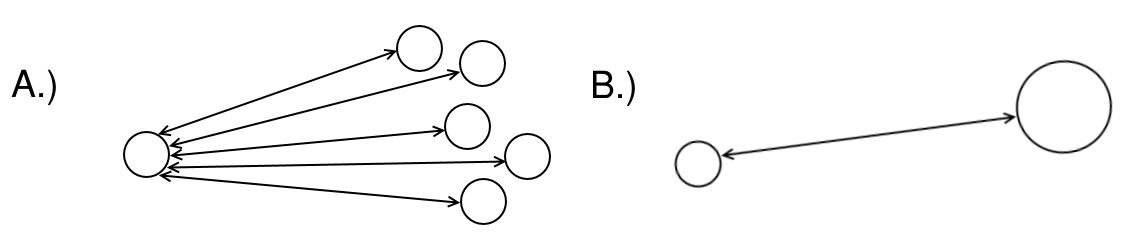
\includegraphics[width=1.0\textwidth]{Figures/SeriesToCluster.png}
\caption{\label{fig:StoC}Distant Elements Approximated to a Single Cluster}
\end{figure}

The series of elements approximated to a single element in Figure \ref{fig:StoC} is only valid when the convection of the leftmost element is to be performed. For example, the cluster grouping shown could not be used to convect an element inside the cluster group. Hence every element represents a unique situation with its own unique cluster groupings. However, the calculation of these unique cluster groupings represents a large computational overhead, and thus is not beneficial as a method of optimization.
\\\\
To overcome the large computation overhead associated with calculating unique cluster groupings for individual elements a method is used where the cluster groupings are selected based upon groupings which are applicable to most elements. For example, consider figure \ref{fig:ThreeClusters}. Here 3 sets of closely spaced elements can be seen, clustered into the groups A, B and C.

\begin{figure}[H]
\centering
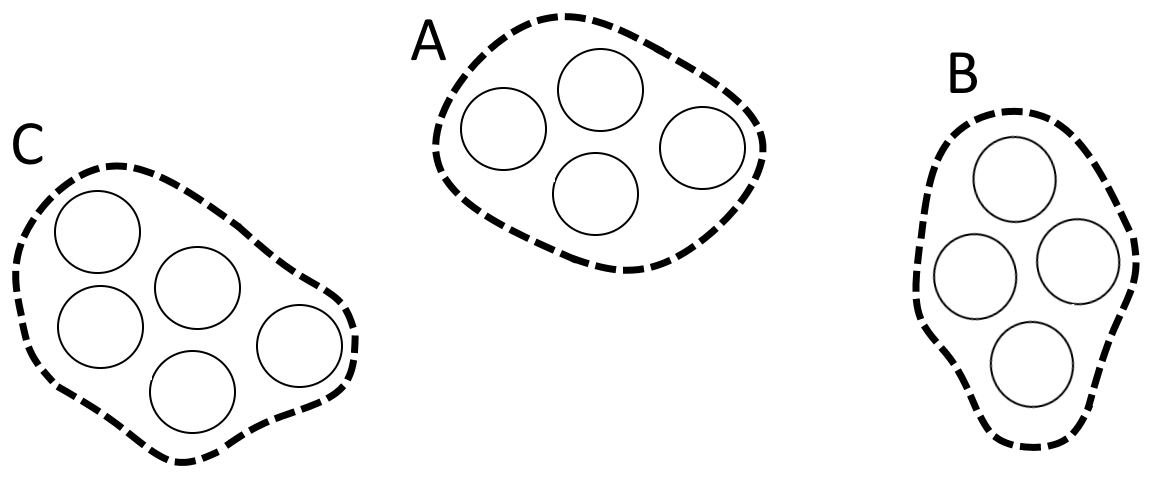
\includegraphics[width=0.6\textwidth]{Figures/ThreeClusters_Example.png}
\caption{\label{fig:ThreeClusters}Closely Spaced Elements and their Respective Cluster Groupings}
\end{figure}

Of course, these cluster groups cannot be used to convect any of the elements, as all elements are in clusters. However, when a single element is to be convected, it could be convected with all elements in its own cluster, and all clusters except its own. This way every element is convected by every other element either directly or through a cluster. Consider for example an element inside cluster B, its convection in this manner is demonstrated in figure \ref{fig:EinB}

\begin{figure}[H]
\centering
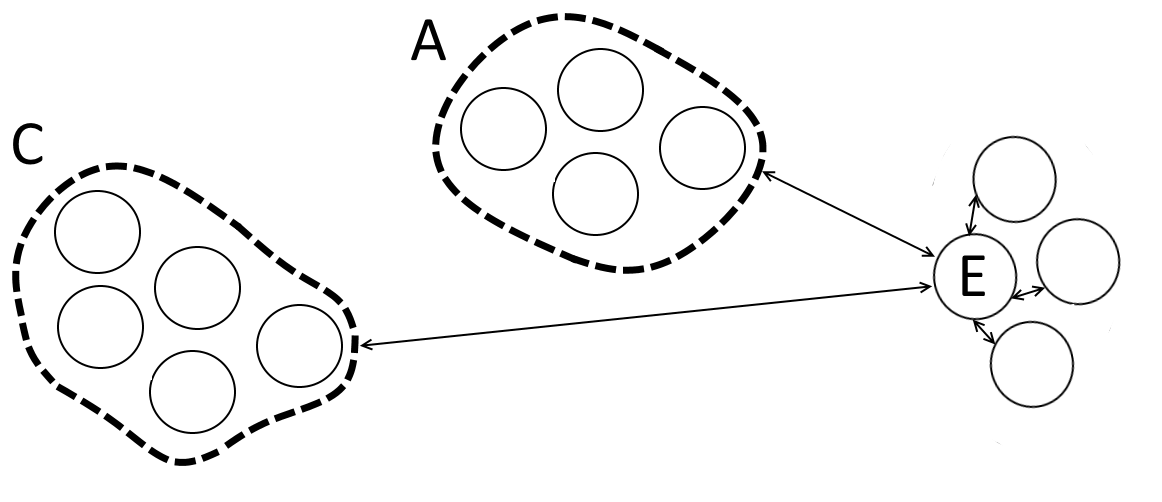
\includegraphics[width=0.6\textwidth]{Figures/ElementInB.png}
\caption{\label{fig:EinB}Element 'E' in cluster 'B' Convecting with Individual Elements and Clusters}
\end{figure}

In figure \ref{fig:EinB} an element "E" from cluster B is shown being convected in the previously discussed way. Consider all elements in cluster C, if they are convected in this manner they will be convected by clusters A and B. Hence, the elements in B and A will both convect with cluster C. Likewise elements from clusters C and A will have cluster B in common. In this way clusters may be calculated once for all elements and still be applicable, despite each element requiring a unique situation.
\\\\
If clusters A and B were closer together it may not be beneficial to convect individual elements in B with the cluster of A but instead with the individual elements of A. Neither is it necessary to convect the elements in cluster B with cluster A, an evaluation based on distance and vorticity could be made to determine whether it would be best to take into account close clusters as a cluster or their constituent elements.
\\\\
Approximating a series of elements to a cluster imposes a degree of error as those individual elements are assumed to act at the position of the cluster rather than their actual positions. This error is unavoidable however its magnitude can be reduced by proper cluster grouping and by more accurate ways to determine cluster position.

\subsubsection{Fixed Cluster Scaling}
A fixed cluster scaling scheme is the simplest clustering scheme considered in this report. The scale of the cluster is used here not to refer to the amount of elements in the cluster. The amount of elements in a cluster is determined by the spatial positioning of the elements. Rather, the scale of a cluster refers to the way clusters are combined to create new clusters. Up until this point clusters comprised solely of elements have been considered, however a situation could be  envisaged where with increased distance from a series of clusters, those clusters could be further clustered together to create a cluster comprised of clusters. This is demonstrated in figure \ref{fig:ClustClust} where situation A represents two distant clusters convecting with a given cluster and situation B represents the same situation where the two distance clusters are clustered together.

\begin{figure}[H]
\centering
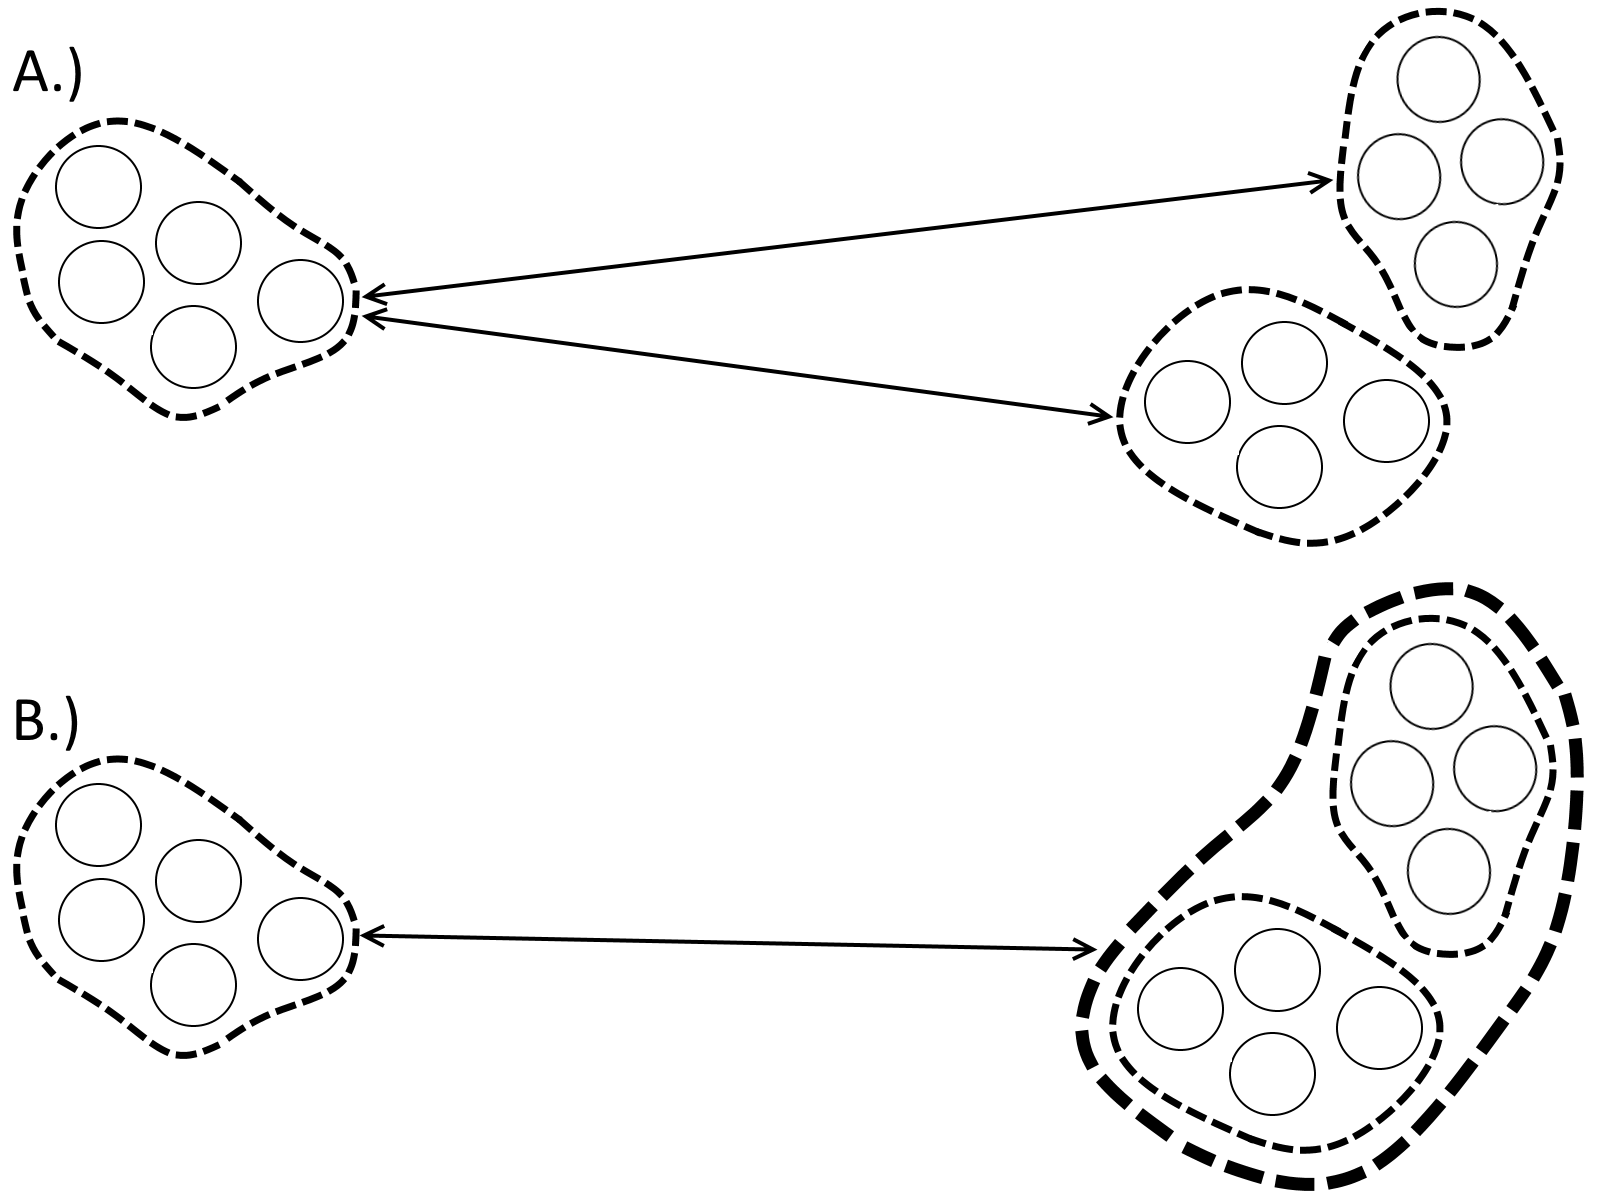
\includegraphics[width=0.5\textwidth]{Figures/ClusterCluster.png}
\caption{\label{fig:ClustClust}Example of Clustering Clusters Together}
\end{figure}

In a fixed cluster scaling scheme clusters are clustered together. Conversely, in a dynamic cluster scaling scheme clusters are clustered together where appropriate to create clusters of clusters.
\\\\
In a fixed cluster scale scheme the clusters are determined via the spatial position of the elements. For the cluster groups to be useful they must be comprised of elements clustered together because they are spatially close together, this gives rise to a physical size of the cluster. In the present simulation, elements are created in a line equidistant to each other and released with uniform velocity perpendicular to the spawn line. Thus the 
elements form a roughly grid shaped pattern as shown in figure.
\\\\
Because the elements form a grid shaped pattern with roughly equal $x$ and $y$ grid spacing the element count in a cluster is fixed, giving rise to the cluster size $N_{Cluster}$. The Biot-Savart law is required to be iterated for all clusters except the cluster the element in question is contained within,  every element from this cluster must be taken into account, the computational cost of convecting a single element is given in equation \ref{eq:clust1}

\begin{equation}
\label{eq:clust1}
C_{Element}=A\frac{N}{N_{Cluster}}+A(N_{Cluster}-1)
\end{equation}

The first term in equation \ref{eq:clust1} represent the computational cost of iterating the Biot-Savart law for all the clusters. Likewise, the second term represents the computation cost of iterating the Biot-Savart law for the individual elements in the element in questions cluster. The computational cost for convecting all elements present is therefore given by equation \ref{eq:clust2}, the term $C_{Cluster}$ is the computational cost of calculating the cluster groupings every loop.

\begin{equation}
\label{eq:clust2}
C_{All}=NA\Big(\frac{N}{N_{Cluster}}+(N_{Cluster}-1)\Big)+C_{Cluster}
\end{equation}

Equation \ref{eq:clust2} can be rearranged to equation \ref{eq:clust3}

\begin{equation}
\label{eq:clust3}
C_{All}=\frac{AN^2}{N_{Cluster}}+AN(N_{Cluster}-1)+C_{Cluster}
\end{equation}

From equation \ref{eq:clust3} it is apparent that the increase in complexity of the scheme still increases proportional to $ON^2$ as in the unclustered case. However the leading term for the fixed scale cluster scheme is proportional to $AN^{-1}_{Custer}N^2$ compared to the unclustered case where complexity rises with $AN^2$. This necessarily represents an optimization, assuming $C_{Cluster}$ is suitable low, as $N_{Cluster}>1$ and in practice takes a value of around 10.

\subsubsection{Dynamic Cluster Scaling}
As aforementioned, clusters were determined dependant on their spatial locations. This resulted in clusters that were widely applicable to all elements. As distance between an element and a series of given cluster increases these clusters will still be applicable, however with increased distance the accuracy lost from clustering together these clusters  reduces, so it is computationally beneficial to treat the series of clusters as a single cluster, again with an equivalent strength and position.

\begin{figure}[H]
\centering
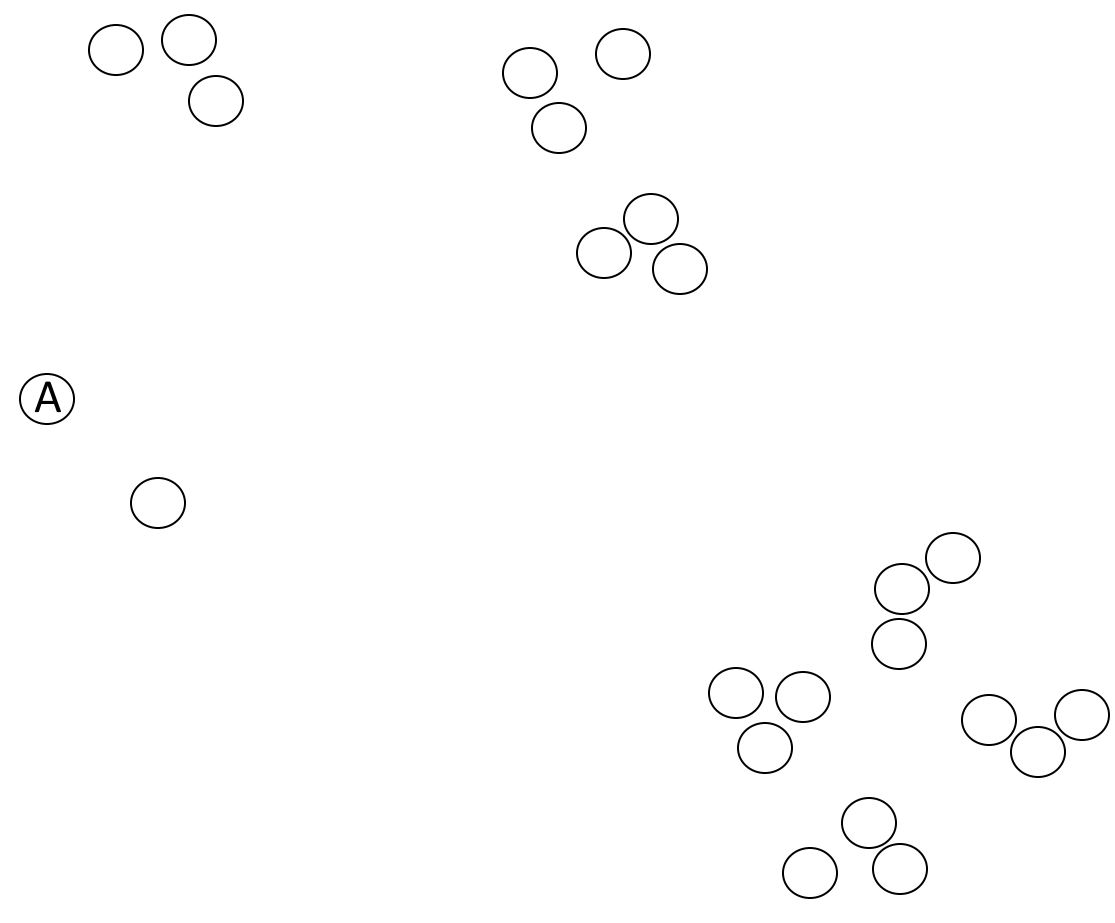
\includegraphics[width=0.45\textwidth]{Figures/LargeSeriesElement.png}
\caption{\label{fig:UnDynClust}Situation of Unclustered Elements}
\end{figure}

To demonstrate this, consider element A in figure \ref{fig:UnDynClust}. Element A must currently convect with all other elements in the situation. However, most of the elements in the scene can be seen to occur in groups of 3, using these groups as the basis for clustering elements, the situation reduces to figure \ref{fig:UnDynClust} 

\begin{figure}[H]
\centering
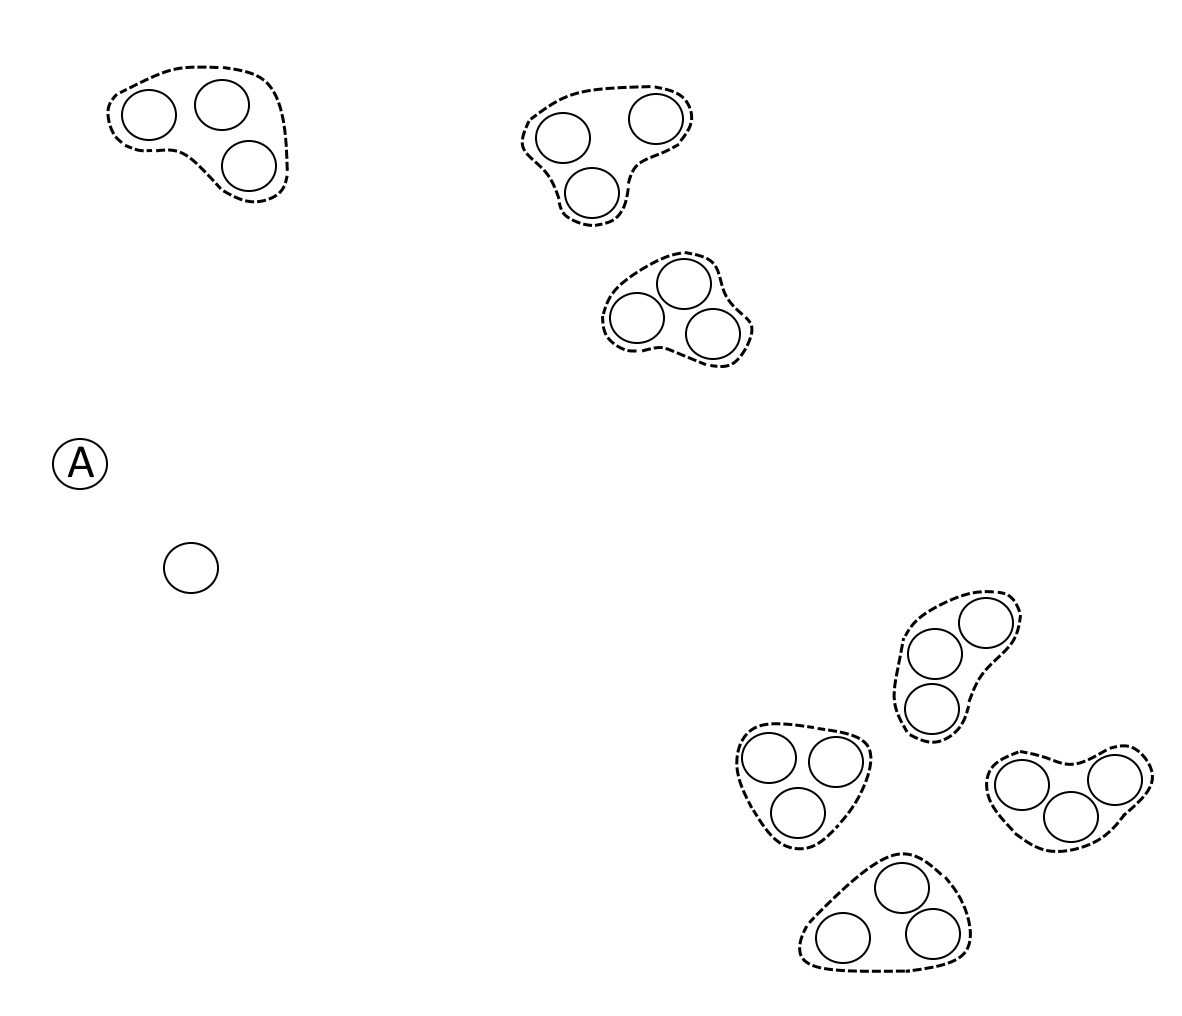
\includegraphics[width=0.45\textwidth]{Figures/LargeSeriesElementFirstCluster.png}
\caption{\label{fig:UnDynClust}Fixed Cluster Size Applied to Situation}
\end{figure}

In figure \ref{fig:UnDynClust} a situation is shown where a fixed cluster scale has been applied. Where as A originally had to convect with 22 separate elements, it must now convect with 1 element and 7 clusters. This can be reduced further by applying a dynamic cluster scaling system, this is shown in figure \ref{fig:DynClust}

\begin{figure}[H]
\centering
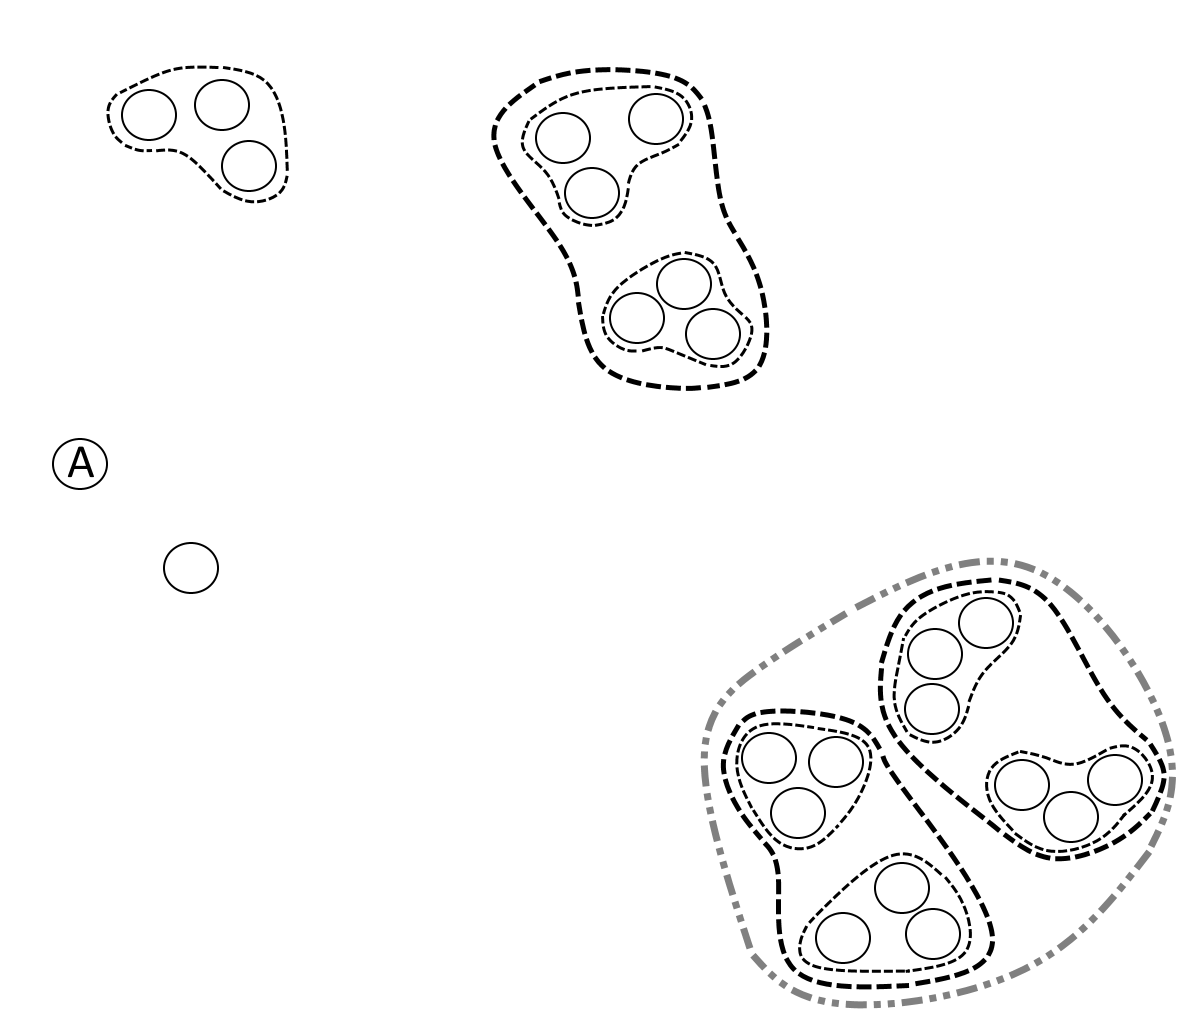
\includegraphics[width=0.45\textwidth]{Figures/LargeSeriesElementSecondCluster.png}
\caption{\label{fig:DynClust}Dynamic Cluster Size Applied to Situation}
\end{figure}

In figure \ref{fig:DynClust} element A now must convect with a single element, a cluster, a cluster of tow clusters and finally a cluster of two clusters, of two clusters. Hence It must convect with 1 element and 3 clusters, a large reduction in computation cost over the original 22 elements. This is an example of dynamic cluster scaling
\\\\
To determine how the computational complexity increases with $N$ first consider the way elements are clustered in figure \ref{fig:ClustDerv}. This shape clustering shape is significant as it is the shape implemented in the DVM, discussed further in section. First two assumptions are made, firstly it is assumed that elements always exist in a perfectly grid shape. Secondly it is assumed that there is a constant cluster size, $\beta$, and elements are clustered into square clusters of $\beta\times\beta$, and clusters of clusters are also clustered into clusters of $\beta\times\beta$. 
In figure \ref{fig:ClustDerv} a series of numbers can be seen be seen next to the grid, this can be thought of as a coordinate system where the unit is iterated every time the end of a cluster is reached spanning a single axis, for brevity this will be referred to as $\varphi$

\begin{figure}[H]
\centering
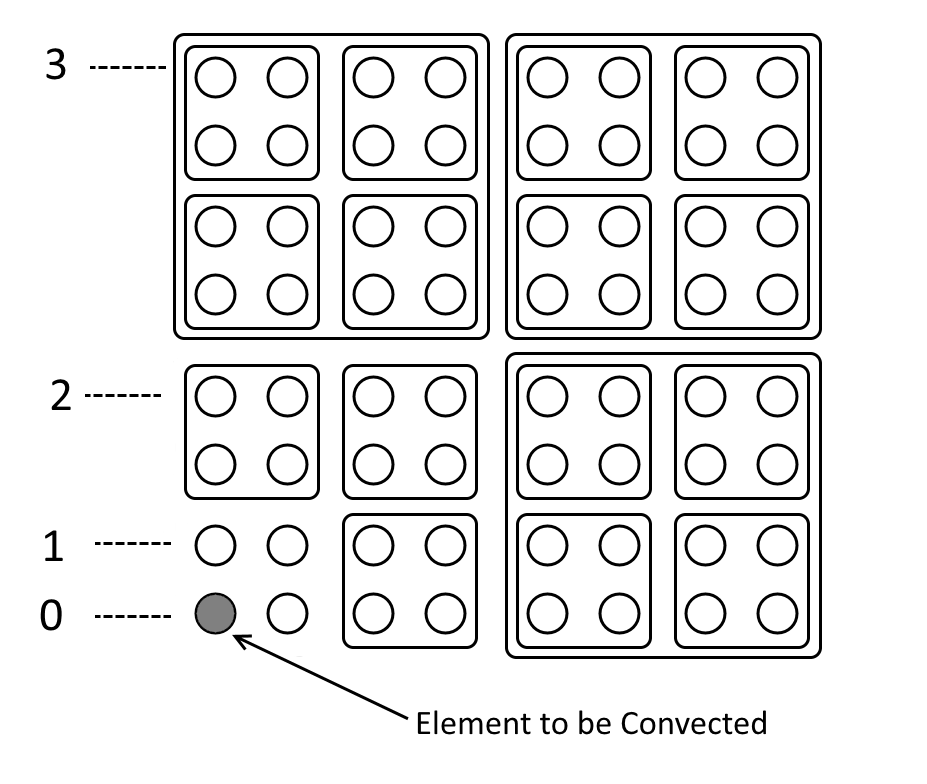
\includegraphics[width=0.55\textwidth]{Figures/DynamicClusterDerivation.png}
\caption{\label{fig:ClustDerv}Dynamic Cluster Size Applied to Situation}
\end{figure}

The first step in deriving the relationship is to consider for every value of $\varphi$ how many elements and clusters are considered, the number of elements and cluster is denoted by $N_{Total}$. As the assumption that clusters always occur in constant sizes of $\beta\times\beta$ then as $\varphi$ is incremented by unity then 3 clusters are added. At a value of $\varphi=1$ there are $\beta\times\beta-1$ elements to convect with (as an element cannot convect with itself). Hence for all non zero positive integers $N_{Total}$ is given by \ref{eq:NoClusts}

\begin{equation}
\label{eq:NoClusts}
N=(\beta^2-1)+3(\varphi-1)
\end{equation}

Expanding the brackets and combining constants into a single constant $C$ in equation \ref{eq:NoClusts} results in equation \ref{eq:NoClusts2} 

\begin{equation}
\label{eq:NoClusts2}
N=C+3\varphi
\end{equation}

This represents the Number of times the Biot-Savart law needs to be performed, making the assumption that every iteration takes the same computational time, represented by a constant A, an expression for the computational cost in terms of $\varphi$ can be found. This is shown in equation \ref{eq:NoClusts5}

\begin{equation}
\label{eq:NoClusts5}
Cost=C+3A\varphi
\end{equation}

Now the number of elements present for every value of $\varphi$ needs to be found. Consider the position along a single dimension of the square for each value of $\varphi$. In the example shown in figure \ref{fig:ClustDerv} the values of $\varphi = 1, 2, 3$ refer to positions $2,4,8$ along a single dimension of the grid. In general then the position is given by $\beta^\varphi$. Hence the amount of elements present as a function of $\varphi$ is given by equation \ref{eq:NoClusts3} 

\begin{equation}
\label{eq:NoClusts3}
N_{E}(\varphi)=(\beta^\varphi)^2=\beta^{2\varphi}
\end{equation}

Equation \ref{eq:NoClusts3} can then be arranged to find $\varphi$ in terms of the total number of elements. This is shown in equation \ref{eq:NoClusts4}

\begin{equation}
\label{eq:NoClusts4}
\varphi=\frac{1}{2}\log_{\beta}(N_E)
\end{equation}

Substituting the value of $\varphi$ from equation \ref{eq:NoClusts4} into equation \ref{eq:NoClusts5} yields an equation for the computational cost in terms of the number of elements, this is shown in equation

\begin{equation}
\label{eq:NoClusts6}
Cost=C+\frac{3}{2}\log_{\beta}(N_E)
\end{equation}

In equation \ref{eq:NoClusts6} it can be seen that  the cost increases proportional to $O\log(N)$.

\subsubsection{Reactive Cluster Grouping}
As previously discussed, predictively grouping clusters may not suffice for all conditions. If this is true clusters must be grouped reactively based upon their current positions. This necessarily introduces an overhead associated as groupings must be calculated periodically.
\\\\
The simplest reactive method of calculating cluster groupings splits the spatial domain into a grid where each grid segment represents a cluster, this is shown in figure \ref{fig:GridClust}.

\begin{figure}[H]
\centering
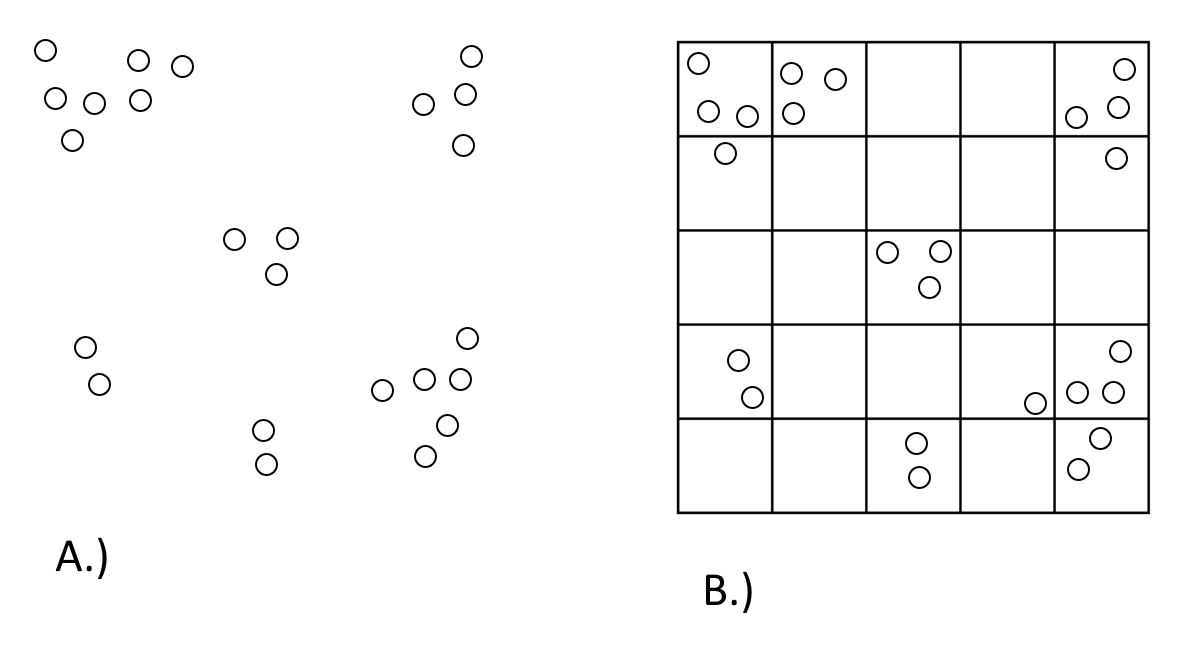
\includegraphics[width=0.65\textwidth]{Figures/Grid_Cluster.png}
\caption{\label{fig:GridClust} Scattered unclustered elements (A) shown with grid based clustering applied (B)}
\end{figure}

In figure \ref{fig:GridClust} a grid has simply been overlaid on a series of scattered elements, in essence this is exactly how the method works, however extended into 3D. Elements inside a given grid segment are assumed to act as part of a cluster.
\\\\
As every element in a given grid space is assumed to be part of a cluster, calculating cluster groupings is easy as only the the coordinates of the element need be taken into account and not which elements are close to a given element. Each cluster grouping may also be identified by a set of coordinates relative to the grid (referring to the placement on the grid, not actual spatial dimensions), this is demonstrated in figure \ref{fig:GridClustCoord}.

\begin{figure}[H]
\centering
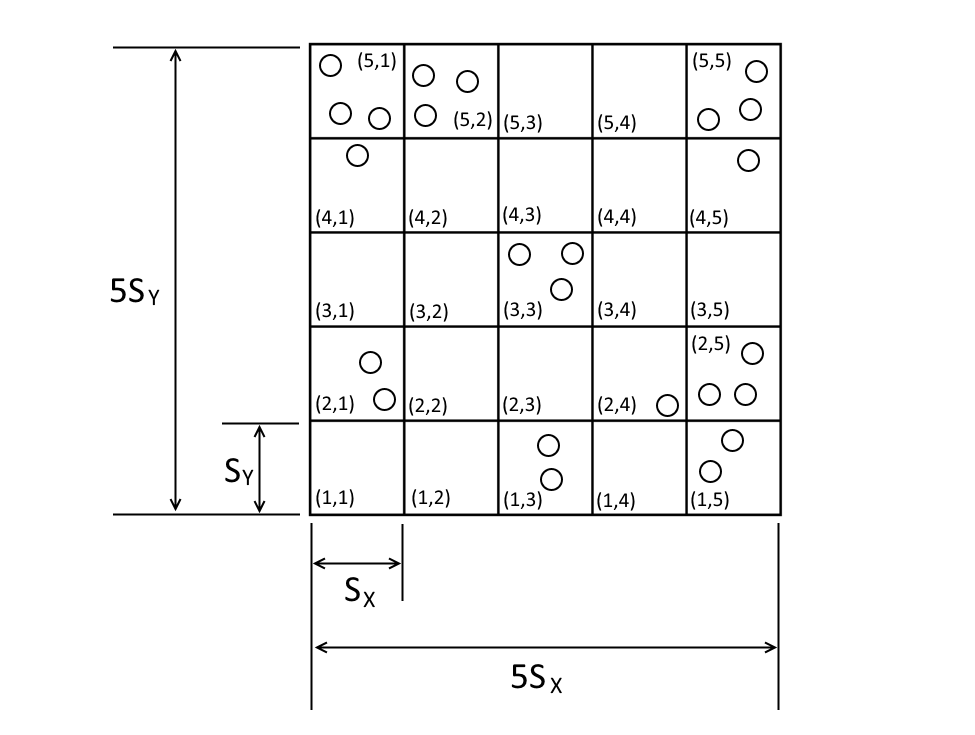
\includegraphics[width=0.65\textwidth]{Figures/GridClustCoord.png}
\caption{\label{fig:GridClustCoord} Grid Based Clustering Coordinate System and Grid Spacing}
\end{figure}

In figure \ref{fig:GridClustCoord} the grid spacings $S_X$ and $S_Y$ are shown. The nomenclature (x,y) is used to specify a given grid cell. Hence determining which cluster and element belongs to in the form $(N_x,N_y)$ is done by evaluating when the conditions in equation \ref{eq:ClustCheckX} and \ref{eq:ClustCheckY} are true.

\begin{equation}
\label{eq:ClustCheckX}
S_x(N_x-1)<P_x\leqslant S_{x}N_{x}
\end{equation}
\begin{equation}
\label{eq:ClustCheckY}
S_y(N_y-1)<P_y\leqslant S_{y}N_{y}
\end{equation}

Clustering elements into such a grid has a second advantage, dynamic cluster scaling is easy to apply. For example, it is easy to cluster grid cells into clusters of 2x2 or 4x4 cells. Further it is easy to determine in advance which cells should be treated as individual elements, clusters and larger order clusters as the spacing of cells is constant. A predefined map of how cells should be treated can be defined, such an example is shown in figure \ref{fig:GridClustering}. In figure \ref{fig:GridClustering} the convection of every element in a single cell (shaded in gray) is considered, as the spatial domain is split into discrete cells of constant spacing, a pattern of cell clustering can be overlaid on its position is valid for any cell in the spatial domain. Using such a method to determine how cells are consider (elements, clusters ect..) avoids having to evaluate clusters based on position and strength reactively.
\begin{figure}[H]
\centering
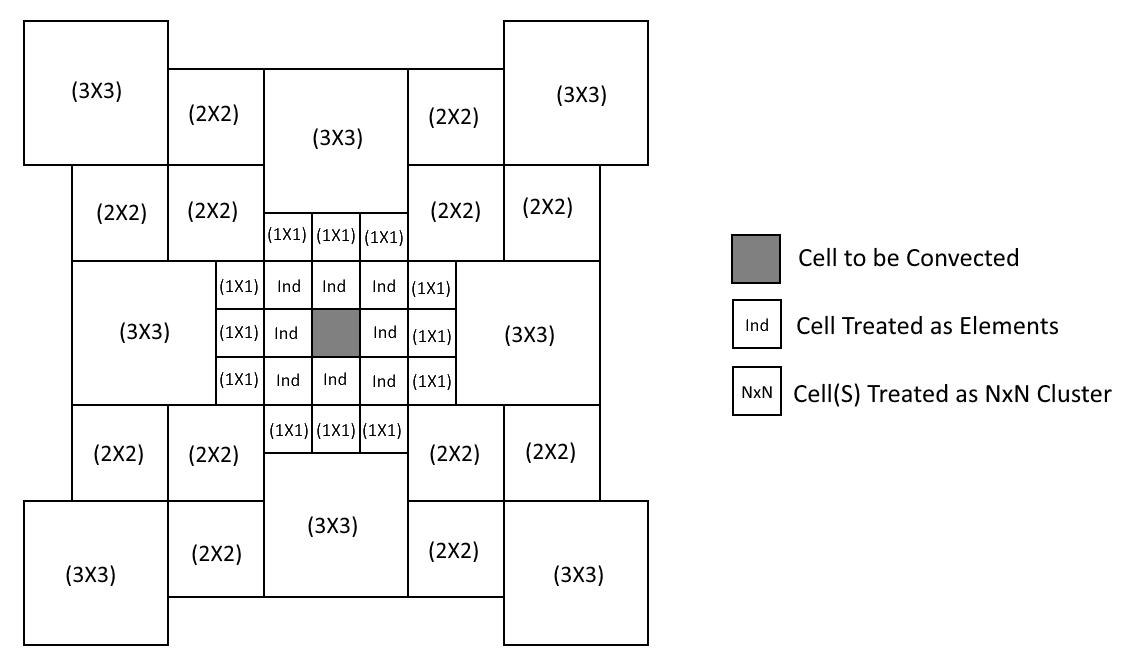
\includegraphics[width=1.10\textwidth]{Figures/CellClustering.png}
\caption{\label{fig:GridClustering} Example of Predetermined Clustering of Grid Cells}
\end{figure} 


\subsubsection{Predictive Cluster Grouping}
Elements are created with equal spacing along the span of the wing, this is demonstrated in figure \ref{fig:ElementLocations} A. Elements travel  away from the aerofoil with the free stream velocity, this is shown in figure \ref{fig:ElementLocations} B.

\begin{figure}[H]
\centering
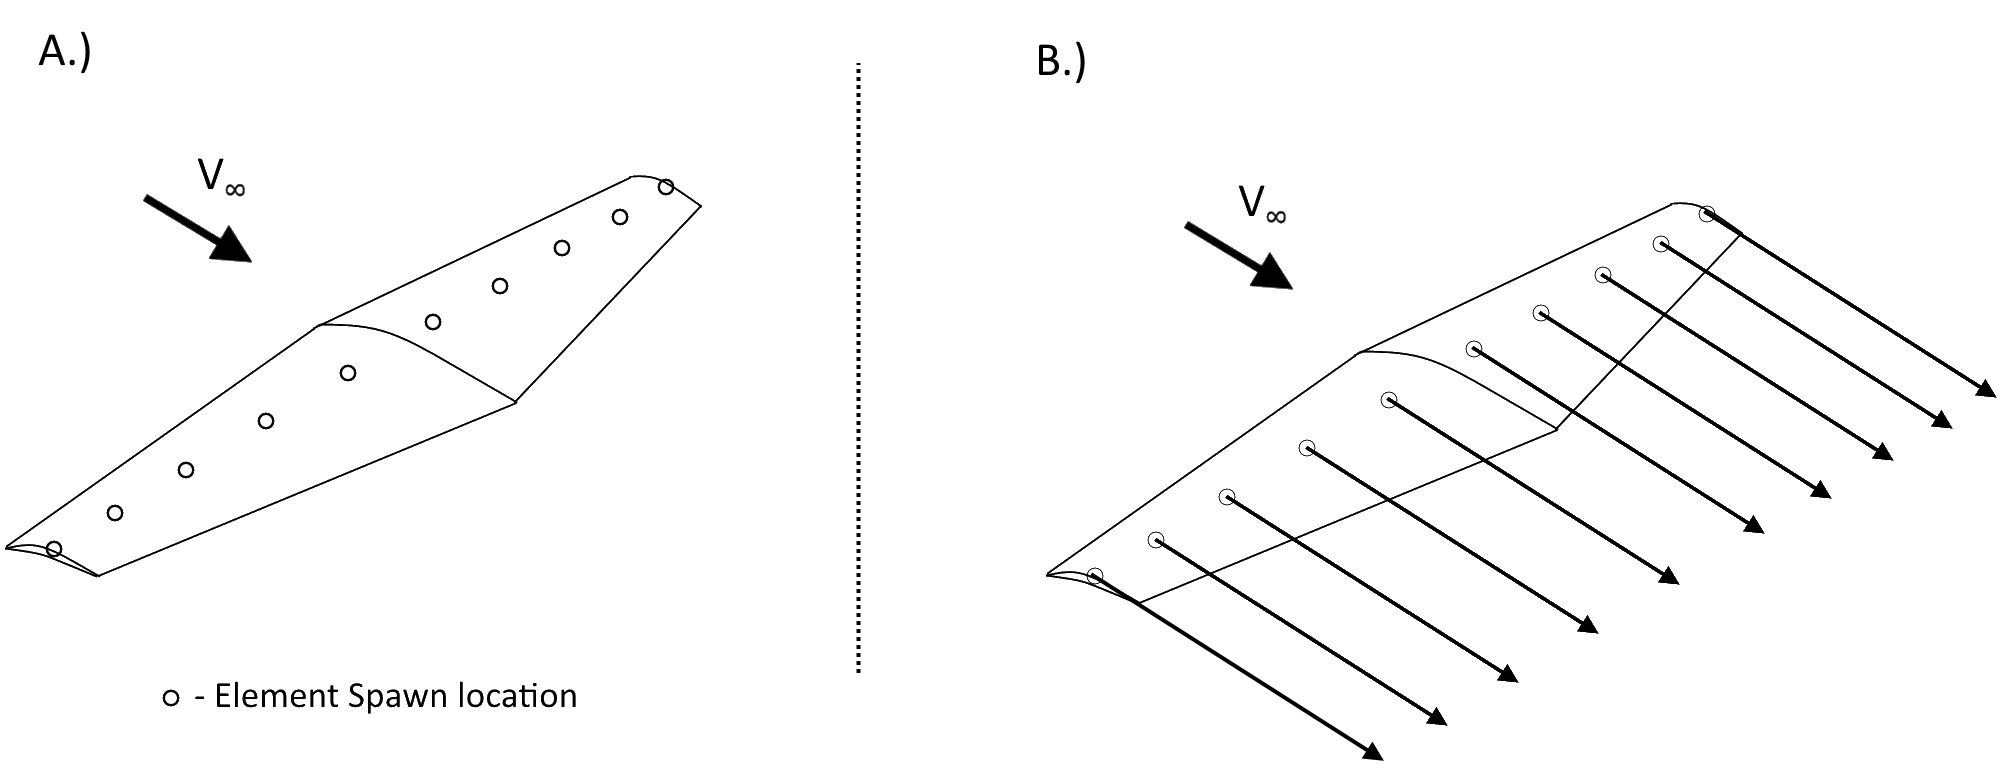
\includegraphics[width=0.9\textwidth]{Figures/ElementSpawnLocations.png}
\caption{\label{fig:ElementLocations} Element Spawn locations along wing span}
\end{figure} 

After a certain time a new row of elements is created, the velocity of the elements in both is roughly the same, this gives rise to a grid shaped pattern of elements, shown in figure \ref{fig:WindGrid}. 

\begin{figure}[H]
\centering
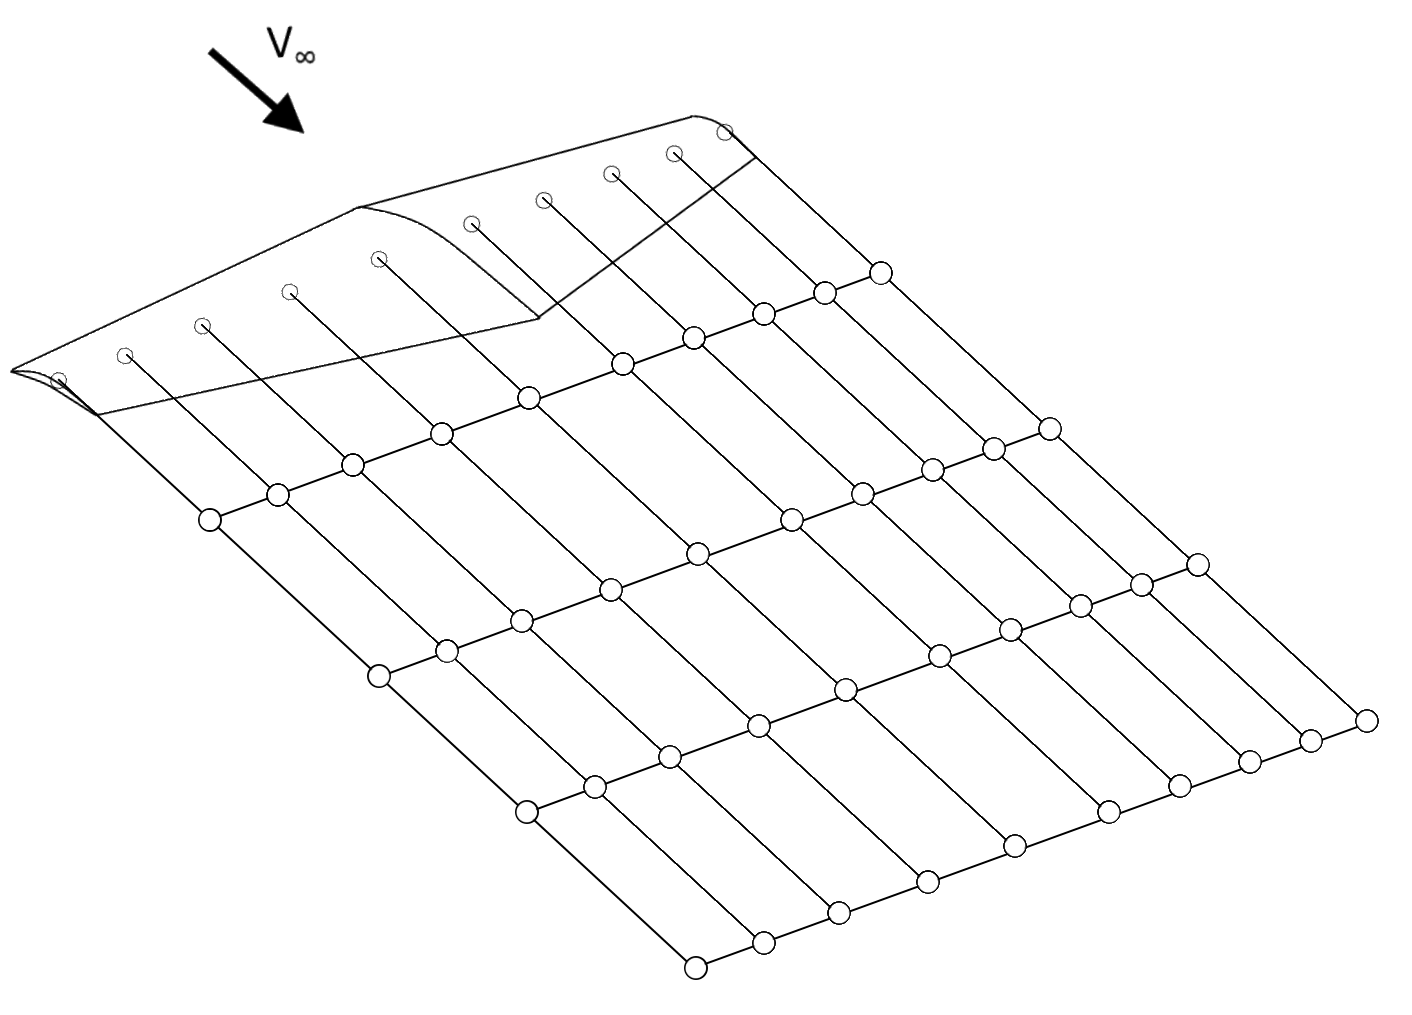
\includegraphics[width=0.7\textwidth]{Figures/WingGrid.png}
\caption{\label{fig:WindGrid} Apparent "Grid" shape Made by Successive Element Rows}
\end{figure} 

This represents a vortex sheet, of course the elements do not stay in a perfectly planar grid pattern, however neighbouring elements do stay close to each other as the sheet rolls up at the sides. Predictively clustering elements assumes that this grid can be assumed to stay in a shape, though changing,where clusters can be predicted based up on the grid shape. As a grid shape is present, pre determined clustering "shapes" such as those seen in figure \ref{fig:GridClustering}.
\\\\
This clustering system becomes inaccurate when this assumption becomes untrue. When strong wingtip vortices are formed, or lift generation is changed suddenly, are both examples of when this assumption leads to poor accuracy. However, this method may be advantageous over the reactive clustering method as it presents no overhead associated with determining cluster groupings 

\subsubsection{Cluster Position}
An error is introduced into a simulation using a clustering scheme as the position of every individual element in a cluster is lost and every element assumed to act the clusters potion. Determining the position of the cluster will therefore have an effect of the magnitude of this error. The simplest approach to calculate a clusters position would be to average the coordinates of all elements in the cluster. This method weights the position of all elements equally in a cluster. In this section two alternative methods are discussed, a weighted average and a simpler highest influence approach.
\\\\
Consider a cluster consisting of an amount $N_{Cluster}$ of elements, the position vector of any given element is $P_{N}$ and its respective vorticity is $\omega_{N}$. To find a weighted average the total vorticity of the cluster is first found, this is shown in equation \ref{eq:clust4}

\begin{equation}
\label{eq:clust4}
\omega_{Total}=\sum^{N_{Cluster}}_{N=1}\omega_{N}
\end{equation}

Every element is asigned a relative weighting $W_{N}$, for the simple average position case this would be constant for all elements and be equal to $N^{-1}_{Cluster}$. This approach weights the potion of the cluster based on the vorticity of each element, the influence of every element is defined as the ratio of its vorticity to the total vorticity of the cluster. This is shown in equation \ref{eq:clust5}

\begin{equation}
\label{eq:clust5}
W_{N}=\frac{\omega_N}{\omega_{Total}}
\end{equation}

Hence the weighted average position of the cluster is given by equation \ref{eq:clust6}

\begin{equation}
\label{eq:clust6}
P_{Cluster}=\sum^{N_{Cluster}}_{N=1}\frac{\omega_N}{\omega_{Total}}P_{N}
\end{equation}

The position of clusters are determined only once for every convective cycle, hence the computation overhead of determining their position is minor in comparison to the cyclic convecting routine. Whilst it is true that determining cluster position should not pose a significant slow down of the simulation, the process can be optimized further by using a Highest Influence approach. In such a method, the cluster is assumed to act at the point of the element whose vorticity is the highest of the cluster. As there is no calculation involved in this method, it is significantly more lightweight than both the average and weighted average approaches.








\section{Theory - Temporal Discretization}
\subsection{Introduction}
The convective routine results in the calculation of the velocities of all elements at a given time given a series of element positions and vorticity, solving analytically results in a large number of interdependent differential equations that are problematic and inefficient to solve in real time. Instead the time domain is discretized into discrete “Time Steps” and numerical approximations used to solve for the position of the elements at the end of the time step. Splitting the time domain into discrete time steps is known as “Temporal Discretization”.
\\\\
The problem can be stated as given a current position $X_{1}$, time $t_{1}$ and velocity $v_{1}$, find the position $x_{2}$ at $t_{2}=t_{1}+t_{ts}$. This is shown in equation \ref{eq:tdprob} where $f(v_{1},t_{ts})$ represents the scheme used.

\begin{equation}
\label{eq:tdprob}
x_{2}=x_{1}+f(v_{1},t_{ts})
\end{equation}

The discretization process necessarily introduces discretization error. By approximating the continuous function to a discrete series of  points a truncation error is introduced, this error reduces as more points are used to represent the continuous function. Hence, as a finer time step is used this error will decrease. The way in which this error scales with the time step is known as the order of accuracy of the scheme. The order of accuracy is determined by how the leading error term scales with the time step. For example, in a first order scheme the leading error term is proportional to the time step used squared, this is shown in equation \ref{eq:tdfirstorder}. Likewise, in a second order scheme the leading error term is proportional the the time step cubed, this is demonstrated in equation \ref{eq:secondorder}. Note, these definitions are for schemes applied to differential equations and are not the same as the traditional CFD definitions for order of accuracy.
\begin{equation}
\label{eq:tdfirstorder}
x_{2}=x_{2}+ot_{ts}^2
\end{equation}
\begin{equation}
\label{eq:secondorder}
x_{2}=x_{2}+ot_{ts}^3
\end{equation}

It would then seem that a higher order scheme is preferable as the truncation error is reduced quicker as the time step is refined. However higher order schemes are also associated with a higher computational overhead and diminishing returns from even higher order schemes will become apparent. Further, the truncation error is not the only variable when deciding upon a scheme to use. Two major considerations are made when determining a scheme to use, the convergence and stability of a scheme. As truncation errors sum up as the routine is iterated, the approximated value of the function is seen to "drift" away from the actual value of the function as the approximation diverges. To increase convergence a finer time step or higher order discretization scheme can be used.
\\\\
The rate of convergence of a scheme can be expressed as the rate at which the error norms of the approximation reduces as the time step is refined, a definition of error norms is given in equation \ref{eq:errornormsdef} where $x^{(n)}$ is the numerical approximation to the continuous function and $x^{ex}$ is the exact solution. Convergence of a scheme can be tested by calculating the Error norms of a known continuous function 

\begin{equation}
\label{eq:errornormsdef}
Error^{(n)}=\sum_{n}^{1} |x^{n}-x^{ex}|
\end{equation}

Higher order schemes often decrease the stability of the approximation. Stability issues arise due to the approximation consistently over or underestimating the value of the function, or the scheme producing non-physical results. Higher order schemes are more susceptible to this error as they may produce more extreme fluctuations based on their inputs if those inputs are based only on current and/or previous values of the function and the independent variable, these are known as explicit schemes. However schemes that utilize future values of the function and independent variables, known as implicit scheme, do not exhibit this behavior to a significant degree. 
\\\\
It may seem that a high order implicit scheme would be the best choice for a discretization scheme. And indeed these are the most common schemes employed by real time physics engines. Whilst PhysX (utilized by unity) and other popular physics engines such as Havok and Newton are closed source and so their schemes are not disclosed (PhysX is know to use a implicit simplectic scheme of unknown order) a number of open source engines are available. ODE (Open Dynamics Engine) is a popular open source physics engine, being open source its source code can be freely examined. The Open Dynamics Engine uses an implicit method described by Stewart and Trinkle in their 1996 paper "An implicit time-stepping scheme for rigid body dynamics with inelastic collisions and Coulomb friction".
\\\\
Despite both PhysX and ODE using implicit schemes, an explicit scheme is to be used for this simulation. For PhysX and ODE the use of an explicit scheme is reasonable as the largest computational overhead is not associated with the calculation of a velocity of an element (in the the case of PhysX and ODE the element is a Rigidbody, akin to the Discrete Vortex Element in this simulation) and thus it is practical to do this numerous times per time step. Their largest overheads are associated with processes related to collision detection and force summation. However in the present simulation, the single largest overhead is associated with the calculation of the velocity of an element, to such a degree that the discretization scheme represents almost no overhead. Thus using the convection routine to calculate future velocities of elements would represent a decrease in performance.
\\\\
As the discretization scheme represents a near negligible overhead compared to the convection routine the motivation behind developing a new scheme should not centre majorly on the performance of the scheme but the increase in accuracy of the scheme. Any increase in performance of the scheme may represent a slight increase in performance of the overall simulation. However, an increase in accuracy of the scheme will allow for a coarser time step to be utilized to achieve the same accuracy as the original scheme. This coarser time step allows for more computation time allocated to the convective routine, given more computational time more elements can be calculated. Thus, improving the accuracy of the scheme represents a possible large increase in accuracy by allowing more elements to be used during the simulation.
\\\\
In this section, Eulers method of discretization is presented along with 2 novel explicit methods developed for the present simulation based on extrapolations of interpolating polynomials. These schemes are then assessed for their convergence and stability and a suitable scheme selected for the simulation. Eulers scheme is the only scheme that approximates the future value of the function using only current conditions. This is of importance as explicit schemes may only be used once enough time steps have passed such that the previous values they require can be known, thus Eulers scheme is necessarily used at the start of the simulation if an explicit scheme is to be used.

\subsection{Eulers Method}
The convective routine results in the calculation of the velocities of all elements, Eulers scheme makes the assumption that this velocity is constant throughout the entire time step. So it assumes the downwind velocity of the fluid at the next time step is the current fluid velocity. This is shown in equation \ref{eq:euler1} where $v_t$ is the $v_x$ velocity at the current time step and $t_{ts}$ is the time step.

\begin{equation}
\label{eq:euler1}
x_{new}=x_{current}+\int_{t}^{t+t_{ts}} v_{x}dt
\end{equation}

Solving equation \ref{eq:euler1} leads to equation \ref{eq:euler2}

\begin{equation}
\label{eq:euler2}
x_{new}=x_{current}+v_{x}t_{ts}
\end{equation}

This scheme is applied to all 3 spatial dimensions to obtain a new position vector for every blob, this is shown in vector form in equation \ref{eq:euler3}
\begin{equation}
\label{eq:euler3}
\begin{pmatrix}
x\\
y\\
z
\end{pmatrix}_{new}=\begin{pmatrix}
x\\
y\\
z
\end{pmatrix}_{old}+t_{ts}\begin{pmatrix}
v_x\\
v_y\\
v_z
\end{pmatrix}
\end{equation}

To determine the order of accuracy of the scheme, the scheme in the form given in equation \ref{eq:euler2} is taken. The value for $X_{new}$ is then written as a Taylor series approximation centered on $X_{old}$, this is given in equation \ref{eq:euler4}

\begin{equation}
\label{eq:euler4}
x_{new}=x_{old}+x_{old}^{'}t_{ts}+( \frac{x_{old}^{''}}{2})t_{ts}^2+Ot_{ts}^3
\end{equation}

Taking equations \ref{eq:euler2} from \ref{eq:euler4} yields equation \ref{eq:euler5} 

\begin{equation}
\label{eq:euler5}
0=(x_{old}+x_{old}^{'}t_{ts}+( \frac{x_{old}^{''}}{2})t_{ts}^2+Ot_{ts}^3+...)-(x_{old}+v_{x}t_{ts})
\end{equation}

Equation \ref{eq:euler5} further simplifies to equation \ref{eq:euler6}

\begin{equation}
\label{eq:euler6}
0=( \frac{x_{old}^{''}}{2})t_{ts}^2+Ot_{ts}^3+...
\end{equation}

From equation \ref{eq:euler6} it can be seen that the leading error term is proportional to $t_{ts}^2$, hence Euler's method is first order accurate

\subsection{Quadratic Position Scheme}
This scheme approximates the position at the next time step by use of a polynomial to estimate the position of an element at t+ts. A second second degree polynomial is to be used to interpolate the position of each element. In order to fully define a second degree polynomial 3 values of the polynomial are required. However to ensure the scheme converges on the exact solution, the derivative of the interpolating polynomial should be equal to the derivate of the exact solution. To maintain this condition the polynomial is instead mapped to two known positions, and an extra condition imposed relating its derivative to the velocity at the current time step. These conditions are shown in equations \ref{eq:poly1} to \ref{eq:poly3}. 

\begin{equation}
\label{eq:poly1}
p(t)=At^2+Bt+C
\end{equation}

\begin{equation}
\label{eq:poly2}
p(t-t_{ts})=A(t-t_{ts})^2+B(t-t_{ts})+C
\end{equation}

\begin{equation}
\label{eq:poly3}
p'(t)=2At+B
\end{equation}

Rearanging equations \ref{eq:poly1} and \ref{eq:poly2} for C and equations yields equation \ref{eq:poly4}

\begin{equation}
\label{eq:poly4}
p(t)-At^2-Bt=p(t-t_{ts})-A(t-t_{ts})^2-B(t-t_{ts})
\end{equation}

Equation \ref{eq:poly3} can then be rearanged for B, this is shown in \ref{eq:poly5}

\begin{equation}
\label{eq:poly5}
B=p'(t)-2At
\end{equation}

Substituting the value for B from equation \ref{eq:poly5} into equation \ref{eq:poly4} results in a single equation with only one unknown, A. This is shown in equation \ref{eq:poly6}.

\begin{equation}
\label{eq:poly6}
p(t)-At^2-(p'(t)-2At)t=p(t-t_{ts})-A(t-t_{ts})^2-(p'(t)-2At)(t-t_{ts})
\end{equation}

As equation \ref{eq:poly6} has only one unknown, A, we can solve for A. This is shown in equation \ref{eq:poly7}. Steps ommited from the derivation here are included in the appendix

\begin{equation}
\label{eq:poly7}
A=\frac{p(t)-p(t-t_{ts})-p'(t)t_{ts}}{t*t_{ts}+t_{ts}^2}
\end{equation}

Now A is a known value, it can be used to substitute into the original equations to solve for B and C. Equation \ref{eq:poly5} is used for this as it contains only two unknown, A and B, and A in now known. Now both A and B are known values, equation \ref{eq:poly1} can be rearanged to for an expression for C, this is shown in equation \ref{eq:poly8}

\begin{equation}
\label{eq:poly8}
C=p(t)-At^2-Bt
\end{equation}

A, B and C are now all known values, so a second degree polynomial has been obtained to interpolate the position of an element. The calculation of the coefficients further simplifies if for every iteration of the scheme, the current time is take to be 0. In this case, the equations for the coefficients becomes equations \ref{eq:poly9} to \ref{eq:poly11}

\begin{equation}
\label{eq:poly9}
A=\frac{p(0)-p(-t_{ts})-p'(0)t_{ts}}{t_{ts}^2}
\end{equation}

\begin{equation}
\label{eq:poly10}
B=p'(0)
\end{equation}

\begin{equation}
\label{eq:poly11}
C=p(0)
\end{equation}

The future position of the element is then determined by $p(t_{ts})$, this scheme applied to all 3 spatial dimensions is shown in matrix form in equation \ref{eq:poly12}.

\begin{equation}
\label{eq:poly12}
\end{equation}

Because explicit schemes require knowledge

\subsection{Quadratic Velocity Scheme}
This scheme uses a LaGrange Interpolating polynomial to extrapolate the future velocity trend as a function of time which is then integrated over the time step period for all 3 spatial dimensions to estimate the position at the text time step. The general form of the LaGrange interpolating polynomial is given is equations \ref{eq:lagrange1} and \ref{eq:lagrange2}

\begin{equation}
\label{eq:lagrange1}
p(x)=\sum_{j=1}^{n} P_j(x)
\end{equation}

\begin{equation}
\label{eq:lagrange2}
p_j(x)=f(x)\prod_{k=i, k\neq j}^{n} \frac{x-x_k}{x_j-x_k}
\end{equation}

Given 3 know previous know velocities v1, v2, v3 at t1, t2 and t3 respectively, the velocity-time curve interpolating polynomial is given by equation (3)

\begin{equation}
\label{eq:lagrange3}
p(x)=\frac{(t-t_2)(t-t_3)}{(t_1-t_2)(t_1-t_3)}v_1+\frac{(t-t_1)(t-t_3)}{(t_2-t_1)(t2-t_3)}v_2+\frac{(t-t_1)(t-t_2)}{(t_3-t_1)(t_3-t_2)}v_3
\end{equation}

The time-step between iterations of the convection routine is fixed during the simulation, so the three know previous velocities occur at equally spaced time steps, given a fixed time step of $t_{ts}$, the values of t for which velocities are known are given in equation \ref{eq:lagrange4} where t is is the current time.
\begin{equation}
\label{eq:lagrange4}
v_1=v(t-2t_{ts}), v_2=v(t-t_{ts}), v_3=v(t)
\end{equation}

For each time step a new interpolating polynomial is calculated, and the function integrated over the range t to t+tts, to simplify the calculation the polynomial is instead centred around 0, for this case the known velocities reduces to equation \ref{eq:lagrange5}, this polynomial is integrated over the range 0 to tts.

\begin{equation}
\label{eq:lagrange5}
v_1=v(2t_{ts}), v_2=v(t_{ts}), v_3=v(0)
\end{equation}

Centring the polynomial on 0 reduces the complexity of equation \ref{eq:lagrange3} by removing the term $x_1$, equation \ref{eq:lagrange6} shows equation \ref{eq:lagrange4} with substituted values for $t_1$, $t_2$ and $t_3$

\begin{equation}
\label{eq:lagrange6}
p(x)=\frac{(t+t_{ts})(t+2t_{ts})}{2t_{ts}^2}v_1-\frac{t(t+2t_{ts})}{t_{ts}^2}v_2+\frac{t(t+t_{ts})}{2t_{ts}^2}v_3
\end{equation}

Equation \ref{eq:lagrange6} further simplifies to equation \ref{eq:lagrange7}

\begin{equation}
\label{eq:lagrange7}
p(x)=\frac{v_1}{2t_{ts}^2}(t^2+3t*t_{ts}+2t_{ts}^2)-\frac{v_2}{t_{ts}^2}(t^2+2t*t_{ts})+\frac{v_3}{2t_{ts}^2}(t^2+t*t_{ts})
\end{equation}

This can be expressed as a second degree polynomial of the form of equation \ref{eq:lagrange8}.

\begin{equation}
\label{eq:lagrange8}
p(x)=Ax^2+Bx+c
\end{equation}

Where the coefficients A, B and C are given by equations \ref{eq:lagrange9}, \ref{eq:lagrange10} and \ref{eq:lagrange11} respectively

\begin{equation}
\label{eq:lagrange9}
A=\frac{v_1}{2t_{ts}^2}-\frac{v_2}{t_{ts}^2}+\frac{v_3}{2t_{ts}^2}
\end{equation}

\begin{equation}
\label{eq:lagrange10}
B=\frac{3v_1}{2t_{ts}}-\frac{2v_2}{t_{ts}}+\frac{v_3}{2t_{ts}}
\end{equation}

\begin{equation}
\label{eq:lagrange11}
C=V_1
\end{equation}

The change in position of all the blobs is calculated by the integration of this function over the range 0 to $t_{ts}$, this is shown in equation \ref{eq:lagrange12}

\begin{equation}
\label{eq:lagrange12}
\delta x=\int_{0}^{t_{ts}} v(t)dt=\int_{0}^{t_{ts}} (Ax^2+Bx+c)=\frac{At_{ts}^3}{3}+\frac{Bt_{ts}^2}{2}+Ct_{ts}
\end{equation}

Expanding equation \ref{eq:lagrange12} by replacing the coefficients of the polynomial a, b and c with substitutions from equations \ref{eq:lagrange9} through to \ref{eq:lagrange11} results in equation \ref{eq:lagrange13}.

\begin{equation}
\label{eq:lagrange13}
\Delta x=t_{ts}\left[v_1(\frac{1}{6}+\frac{3}{4}+1)+v_2(\frac{1}{3}-1)+v_3(\frac{1}{6}+\frac{1}{4})\right]
\end{equation}

This scheme is applied for all three spatial dimensions, this is shown in matrix form in equation \ref{eq:lagrange14}

\begin{equation}
\label{eq:lagrange14}
\begin{pmatrix}
x\\
y\\
z
\end{pmatrix}_{new}=\begin{pmatrix}
x\\
y\\
z
\end{pmatrix}_{old}+t_{ts}\begin{bmatrix}
v_{x1}	&	v_{x2}	&	v_{x3}\\
v_{y1}	&	v_{y2}	&	v_{y3}\\
v_{z1}	&	v_{z2}	&	v_{z3}
\end{bmatrix}\begin{pmatrix}
\frac{1}{6}+\frac{3}{4}+1\\
\frac{1}{3}-1\\
\frac{1}{6}+\frac{1}{4}
\end{pmatrix}
\end{equation}










\section{Methods}
\subsection{Unity Implementation}
The simulation is programmed in Unity using C-Sharp. C-Sharp is an object orientated programming language developed by Microsoft as part of its .NET program. However Unity implements the language through the Mono platform, this allows for Multi platform development, so the simulation can run on all x86 operating systems and some ARM based systems such as Android and IOS. The language is designed to be inherently similar to C or C++ to aid portability of code between the two languages, the performance of these languages is also comparable. The use of C-Sharp was selected over other languages, such as Matlab, as it poses far high performance and features such as multi-threading, however this is at the cost of a less user friendly languages not orientated for scientific use. Unity utilizes the open source OpenGL API as its rendering engine, as such the visual aspects of the simulation are handled quite naturally by Unity's internal functions. These functions form all user-interface and visualization aspects of the simulation. Whilst originally used, Unity's inbuilt physics engine, PhysX, is not utilized as it represented increased computational overhead for no increase in accuracy.
\\\\
Unlike a traditional procedural style 

\subsection{Simulation Architecture}
The simulation is broken into 4 independant segment

\subsection{Clustering Methods}

\subsubsection{Biasing Scheme}

\subsubsection{Clustering Schemes}

\subsection{Discretization Schemes}
To asses the accuracy of the proposed schemes approximations were made to a known function. The selection of a known function to approximate is problematic as the different schemes have different propensities to model different functions. For example, the Quadratic Position Scheme models the position-time relationship as a quadratic function, thus it will perfectly model such a function. Likewise, the Quadratic Position Scheme models the position-time relationship as a third degree polynomial, and thus would model such a function quite naturally.
\\\\
The function chosen to asses the schemes was $f(x)=e^x-1$, this function was chosen as none of the schemes can naturally model this relationship. A cyclic function such as $f(x)=sin(x)$ was not chosen so that the accumulation of truncation errors could more easily be assessed. As previously discussed, the implicit schemes require information the previous states of the function. Practically this is resolved by using Euler's Method for the required amount of initial iterations. However for evaluation purposes the schemes are seeded with real values of previous states of the known function. This is done so that comparisons can be made on data accountable solely to the individual schemes, the effect of seeding using Euler's method is assessed later.
\\\\
To model the function $f(x)=e^x-1$ using the schemes an initial value of the function at $x=0$ was given, resulting in $f(x)=0$. A value for the derivate at $f(0)$ was given and is analogous to the velocity at the current time step. Using this information (and previous information for the implicit schemes) the schemes are used to make a prediction for the value of $f(t_{ts})$. The value of $f(t_{t})$ approximated by the schemes refers to an actual value of $f(x)$, the $x$ value this value of $f(x)$ refers to is then taken and used to find the value of $f'(x)$ at this point and this is used as the current velocity, and the process is then repeated over a set number of iterations.
\\\\
Approximations were made to $f(x)=e^x-1$ over the range $0\leqslant x \leqslant 4$, over this range the schemes were evaluated for 5 different time steps of $t_{ts}=$ 0.125, 0.25, 0.5, 1 and 2.

\section{Appendix}



%now enable appendix numbering format and include any appendices
\appendix
\include{appendix1}
\include{appendix2}

%next line adds the Bibliography to the contents page
\addcontentsline{toc}{chapter}{Bibliography}
%uncomment next line to change bibliography name to references
%\renewcommand{\bibname}{References}
\bibliography{refs}        %use a bibtex bibliography file refs.bib
\bibliographystyle{plain}  %use the plain bibliography style

\end{document}
